
%\documentclass{article}
%\usepackage{color}
%\usepackage{graphicx}
%\usepackage{multirow}
%\usepackage{wrapfig}
%\usepackage[export]{adjustbox}
%\usepackage{caption}
%\usepackage{subcaption}
%\usepackage{gensymb}
%\title{Constellation Deployment General Strategy}
%\author{Joan Cebr\'ian, Roger Fraixedas, Marina Pons and Xavi Ti\'o}
%\date{19th October 2016}
%\begin{document}
 %  \maketitle

\section{Launching System}
The aim of this section is the selection of a launching platform. First of all, a review of the available ones on the market is carried out, secondly a small group of launchers is chosen and finally, an optimization is developed in order to find the most suitable system. 
	\subsection{Launch site and vehicle analysis}
Now a days there is such a great amount of launchers available over the world. Nevertheless, most of them are designed for very specific missions. In addition, the space career of a country is usually highly attached to the government, for both economic and political reasons. When searching for a launching system, some parameters have to be taken into an account like payload mass, possible inclination angles, launching site, etc. This analysis only considers those rockets which parameters seem adequate for the Astrea constellation launching.  
\newline
\newline
A general research is done in order to filter all the launchers that can be discarded without any study. The result of this research is that there are seven potential rockets in the market capable of deploying the constellation as well as carrying out the replacement needs. The launchers can be divided in two categories: the powerful ones and the small ones. The first ones are capable of carrying heavy payloads, however they present high operation costs whereas the second ones are way more economic due to the reduced size. In addition, the small rockets are more focused on commercial flights without having to attend governmental issues. 

The following table displays the first seven candidates. 
\newline	
	\begin{table}[h]
	\begin{center}
	\begin{tabular}{|c|c|c|c|}
	\hline
	\bf{ENTERPRISE} & \bf{ROCKET} & \bf{LAUNCHING SITE} & \bf{TYPE}  \\
	\hline 
	Rocket Labs & Electron & North Island (New Zealand) & Light \\
	\hline 
	Kosmostras & Dpner & Baikonur Cosmodrome (Kazakhstan) & Light\\
	\hline 
	Arianespace & Ariane V & Guiana Space Center (French Guiana) & Heavy \\
	\hline
	 Arianespace & Vega & Guiana Space Center (French Guiana) & Light\\
	\hline 
	SapceX & Falcon 9 & USA & Heavy \\
	\hline 
	PLDSpace & ARION-2 & Huelva and Cape Canaveral & Light\\
	\hline 
	LEO Launch and Logistics & - & USA & Light \\
	\hline
	\end{tabular}
	\end{center}
	\caption{List of Launchers}
	\end{table} 	
\newline \newline \newline \newline \newline \newline \newline \newline \newline \newline
	\subsection{Last candidates and selection}
Once this first selection is done, more accurate information is needed so as to reach a reliable conclusion. However, none of these enterprises shows its information on the Internet or any similar divulgation channel with the exception of Arianespace. Thus, all of them must be contacted to get the needed data. The same email is sent to all seven enterprises and several days later, three of them show interest in the Astrea constellation: Rocket Labs, PLDSpace and LEO Launch \& Logistics. Since the other enterprises do not answer the requests and, as a consequence, will not provide the necessary information, they can be directly discarded. Hence, the candidates list is reduced to those three who responded the enquire plus Vega, given that its information is available online. Although the needed data of Ariane V is also known, it is discarded by the fact that it presents high operation costs and it is capable of carrying about 5,000 cubesats 3U when the Astrea constellation will have 168 sats. Therefore, the four remaining candidates are studied in more detail and are subjected to an optimization. 
\newline
\newline
In order to find the most suitable option achieving the project objectives, it is thought to do an evaluation process following the Ordered Weighted Average (OWA) method . First of all, the required parameters for the decision have to be determined. According to the orbit design, the range of inclinations, the number of orbital planes and the range of heights must be taken into an account. Nevertheless, more parameters are needed in order to ensure a reliable result: cost per satellite, frequency of launchings per year and number of satellites deployed per launch. Both range of inclinations and number of satellites per launch act as a restriction due to the following two reasons. First, since orbital plane changes are very expensive and are out of consideration, the minimum number of launchings must equal the number of orbital planes. In addition, being capable of deploying the constellation with the minimum number of launchings is an adequate solution. This turns the number of CubeSats per launch into a restriction: the chosen launcher must be capable of launching at least the number of satellites in an orbital plane. Secondly, the inclination is considered a restriction by the fact that if a rocket is not capable of deploying a satellite in the desired inclination, it makes no sense to use it. 

Since the number of orbital planes is 8 and the inclination is 72$^{\circ}$, any launcher which doesn't fulfills one of this restrictions can be automatically rejected. 
\newline
\newline
 Moreover, the following table contains all the information mentioned above which is helpful to compare the different launchers and see if they accomplish the basic features. 
\newline	
	\begin{table}[h]
	\begin{center}
	\begin{tabular}{|c|c|c|c|c|}
	\hline
	 \bf{Parameters} & \bf{Rocket Lab} & \bf{PLD} & \bf{LEO L\&L} & \bf{Vega}\\
	\hline 
	\bf{Satellites/Launch} & 24 & 34 & 150 & 325 \\
	\hline 
	\bf{Inclination($^{\circ}$) } & {39.2 to 99} & {116 or 140} & {any} & {any}\\
	\hline 
	 \bf{Cost/Satellite (US dollars)} & 240,000 & - & 266,667 & 100,000\\
	\hline 
	\bf{Orbital planes} & 1 & 1 & 1 & 1 \\
	\hline 
	\bf{Frequency/year} & 9 & 8 & 8 & 2 \\
	\hline 
	\bf{Range of heights (km)} & LEO & LEO & LEO & LEO\\
	\hline
	\end{tabular}
	\end{center}
	\caption{Criteria}
	\end{table} 
\newline
\newline
It is important to point out that all the rockets available in the market can achieve the necessary amount of satellites per launch. Although all of them reach the height the CubeSats need, PLD does not attempt the inclination needed which is 72$^{\circ}$. As a result, this launcher is not appropriate for the project purpose and it is rejected. 
According to the remaining 3 candidates, all of them are adequate candidates, nevertheless there is a characteristic that may interfere with the mission goals. At first instance, the frequency per year has not been considered a critical parameter. Those have been chosen regarding orbital parameters only, however, although the frequency does not influence de capability of the rocket of deploying a CubeSat in the desired orbit, it can compromise the set up of the constellation and the posterior replacements. The lower the frequency is, the slower the deployment will be. Therefore, the frequency of the three remaining candidates must be analyzed. As seen in the table, Vega presents the lowest frequency (two launchings per year). This value is not acceptable due to the intention of deploying one single orbital plane per launch. The placement of the whole constellation would last four years, this mean that de first planes would be near their replacement time while the last ones would only have been nearly a year in orbit. Thus, Vega can also be discarded. 
\newline
This leaves the selection with only two options: Rocket Lab and LEO Launch\&Logistics. An Ordered Weighted Average can be made between those two candidates taking the cost/satellite, the number of orbital planes, the frequency and the range of heights into account. Yet, they both present the same number of planes and range of heights, consequently the OWA can be done regarding only the two cost and frequency. The first has to be minimized and the second maximized. Since Rocket Lab presents best values in one parameter and the other (240,000 US dollars vs 266,667 and 9 launchings/year vs 8) there is no need to develop an OWA. In addition, an e-mail from Rocket Lab is received stating that a launch per week is achievable. Thus, the chosen rocket is Electron, from Rocket Lab enterprise. This rocket fulfills all the requirements of the constellation. 
\newline
\begin{figure}[h!]
\centering 
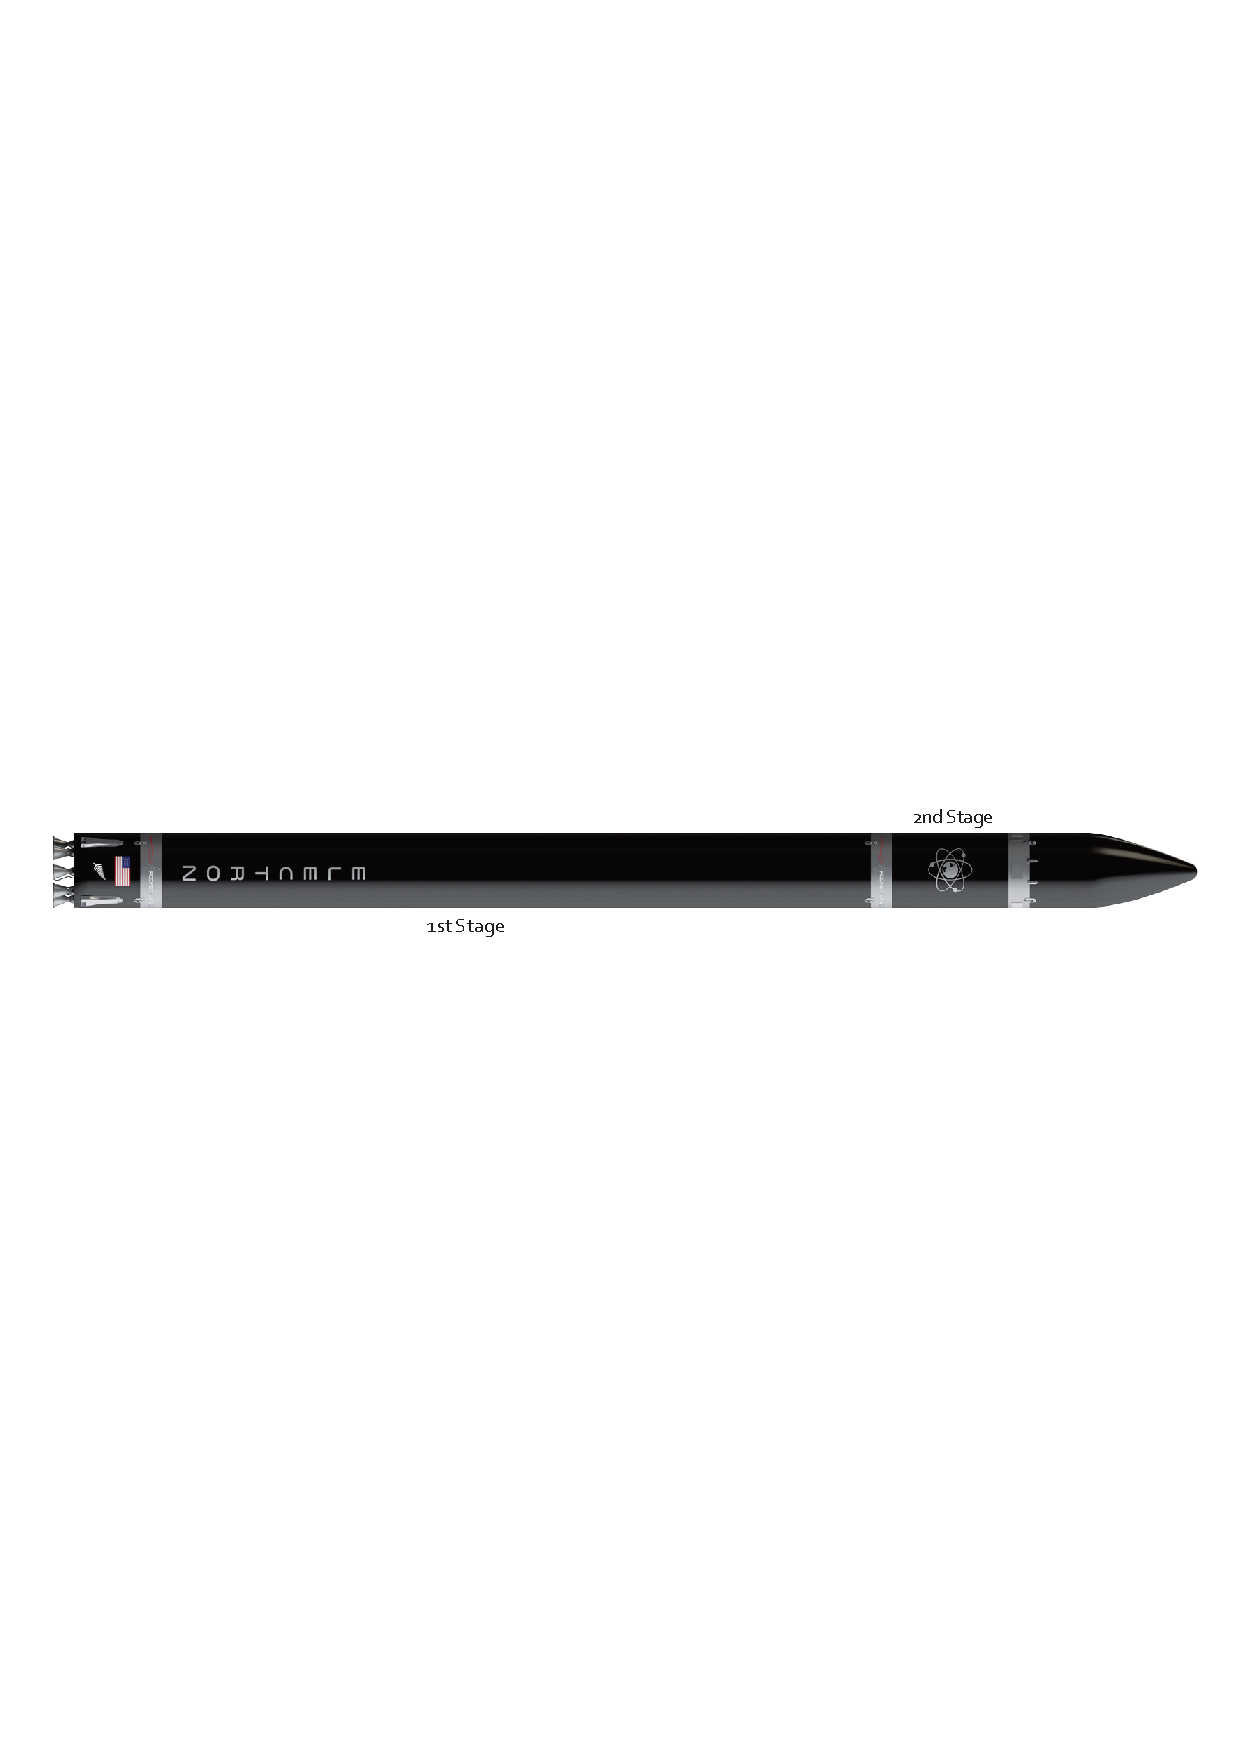
\includegraphics[scale=0.7]{./sections/Constellation_Deployment/S2-Launcher/Images_S2/Picture_1_S2.pdf} 
\caption{Electron Rocket}
\label{fig:rocket}
\end{figure}
\newline
	\subsection{Launcher overview}
Following, a brief description of Electron is provided. 
\newline
\newline
\begin{wrapfigure}{r}{0.6\textwidth}
\centering 
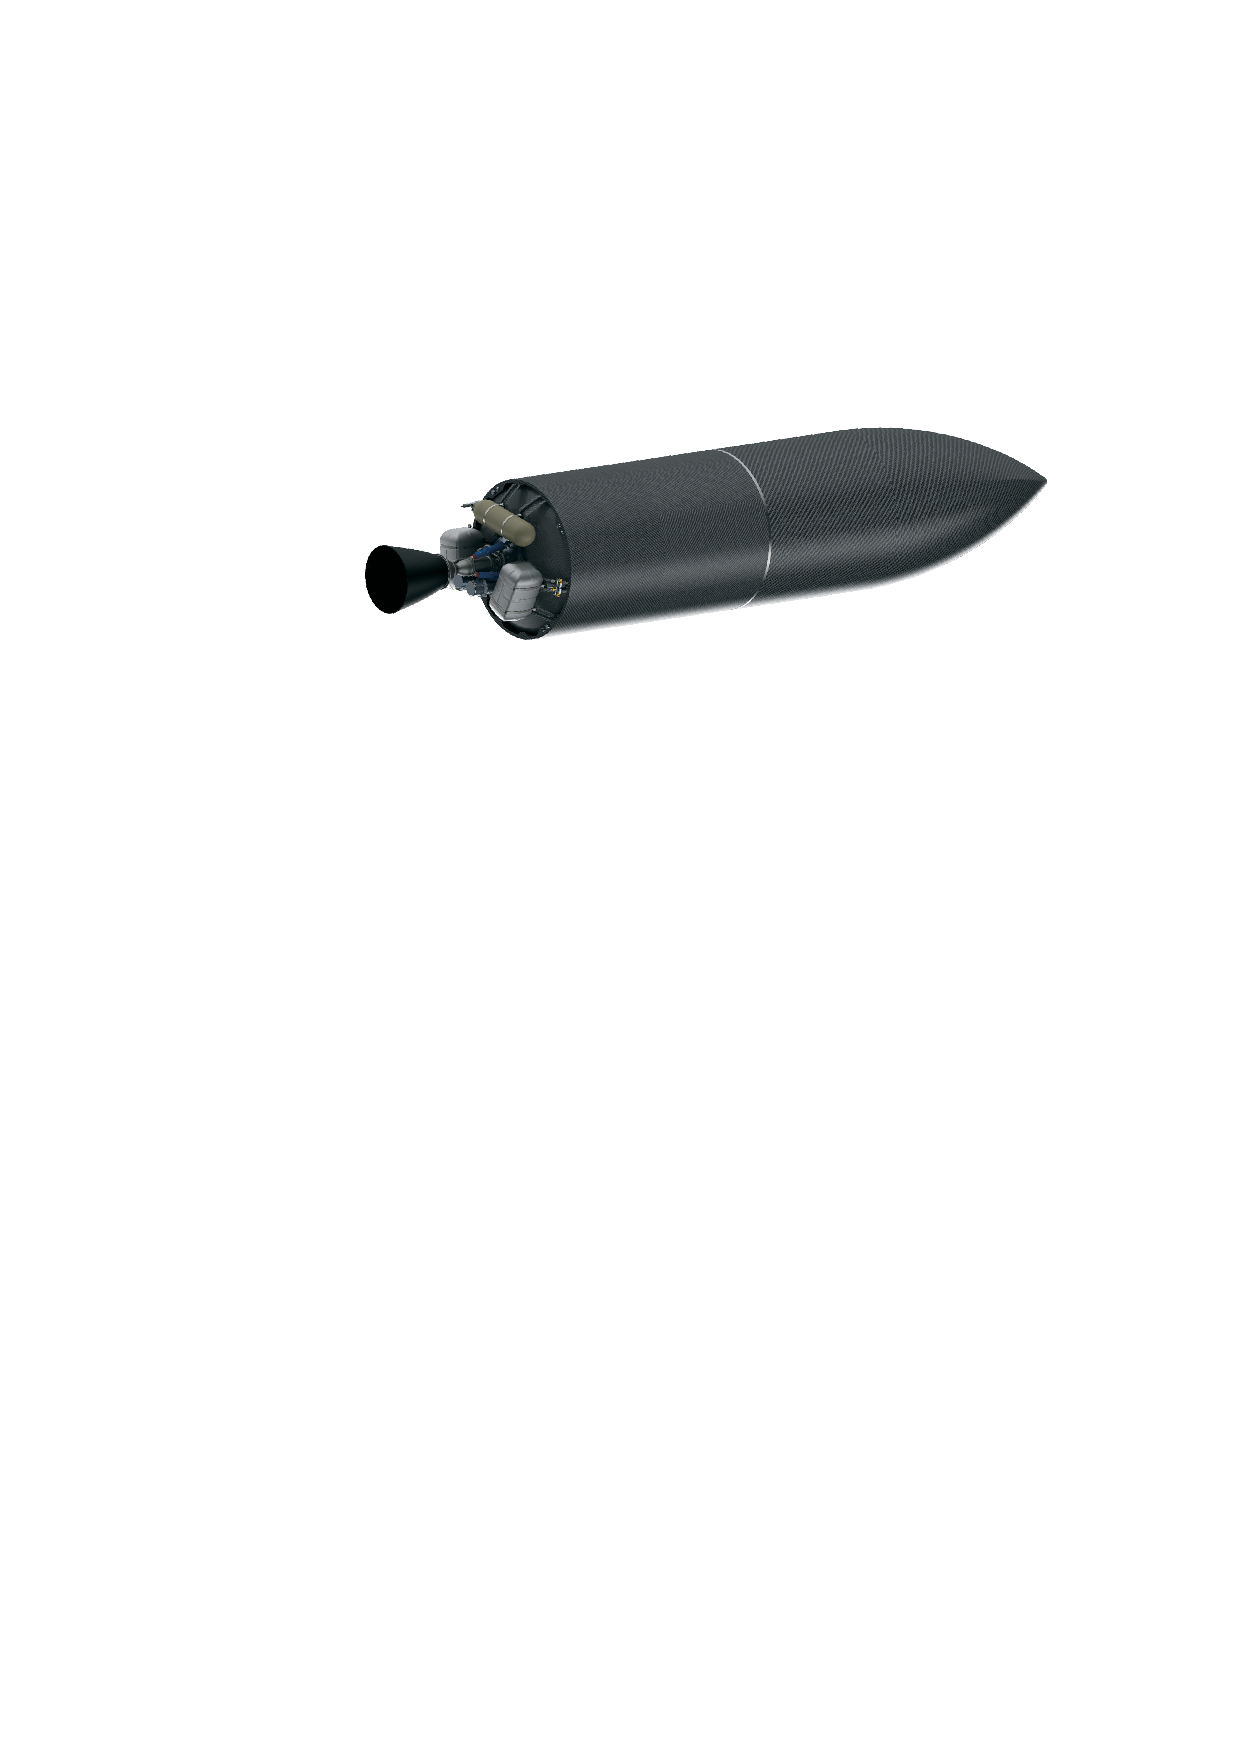
\includegraphics[scale=0.6]{./sections/Constellation_Deployment/S2-Launcher/Images_S2/Picture_2_S2.pdf} 
\caption{Second Stage}
\label{fig:second}
\end{wrapfigure}
Shown in \ref{fig:rocket}, Electron is a two stage light rocket constructed from carbon fiber composite. It is powered by ten Rutherford engines, all of them use liquid oxygen (LOX) and rocket kerosene. The first stage has nine out of the ten engines which generate 152 kN of thrust. The second one, displayed in \ref{fig:second}, has the remaining engine which produces 22 kN. The second stage contains the fairing where the payload is placed. Electron is 17 m long and its diameter is 1.2 m. It is capable of launching 24 3U CubeSats every week at a LEO orbit with a range of inclinations from 39.2 to 99 degrees. 



\newpage
\begin{figure}[h]
\centering 
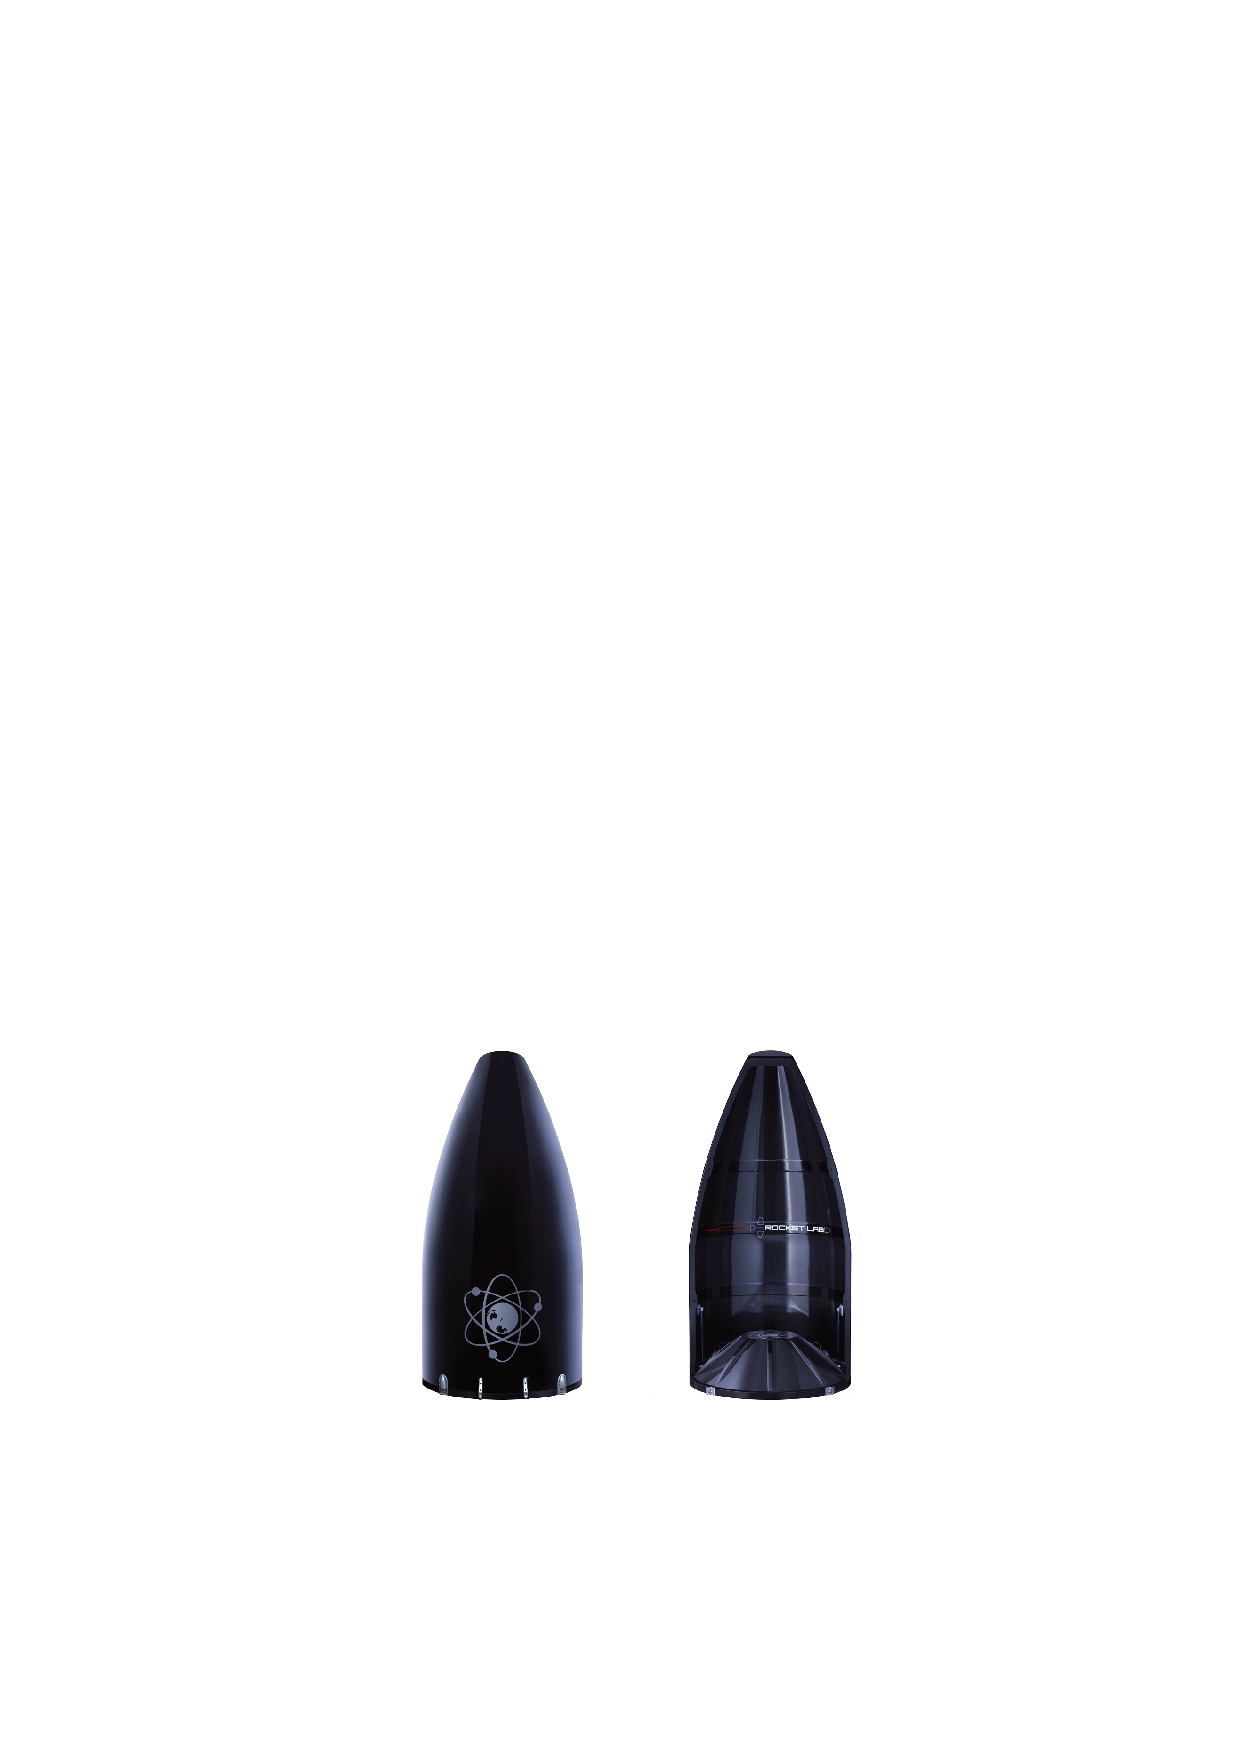
\includegraphics[scale=0.7]{./sections/Constellation_Deployment/S2-Launcher/Images_S2/Picture_3_S2.pdf} 
\caption{Electron Rocket Fairing}
\end{figure}


The injection maneuver is carried out following the flight profile shown in the table 2.3 . The accuracy of the injection is mission dependent, however a typical value would be $\pm15$ Km. 
According to the CubeSat/Fairing interface, Electron is compatible with the standard CubeSat deployers like ISIS or P-POD, in addition, if those deployers are used, Rocked Lab is able to situate the satellites inside the rocket in a more efficient disposition.  
\newline	
	\begin{table}[h]
	% \label{profile}
	\begin{center}
	\begin{tabular}{|c|c|c|}
	\hline
	 \bf{Event} & \bf{Time (s)} & \bf{Altitude (km)} \\
	\hline 
	\bf{Lift-off} & 0 & 0 \\
	\hline 
	\bf{Max Q} & 79 & 11 \\
	\hline 
	\bf{MECO/S1 Separation} & 152 & 69 \\
	\hline 
	\bf{Stage 2 Igintion} & 159 & 69 \\
	\hline 
	\bf{Farinig Separation} & 183 & 110 \\
	\hline 
	\bf{SECO} & 457 & 284 \\
	\hline 
	\bf{Satege 2 Apogee Kick} & 3157 & 499 \\
	\hline 
	\bf{Payload Separation} & 3200 & 500 \\
	\hline 
	\end{tabular}
	\end{center}
	\caption{Flight Profile}
	\end{table} 
\newline


Rocket Lab facilities are located in New Zeland. The test laboratories are placed near the airport of Auckland and the launch site is in Mahia (\ref{facilities}).
\newline
Finally, the cost per satellite is 240.000 US dollars or if the rocket is totally filled, 5.760.000 US dollars the entire launch. 
\begin{figure}[h!]
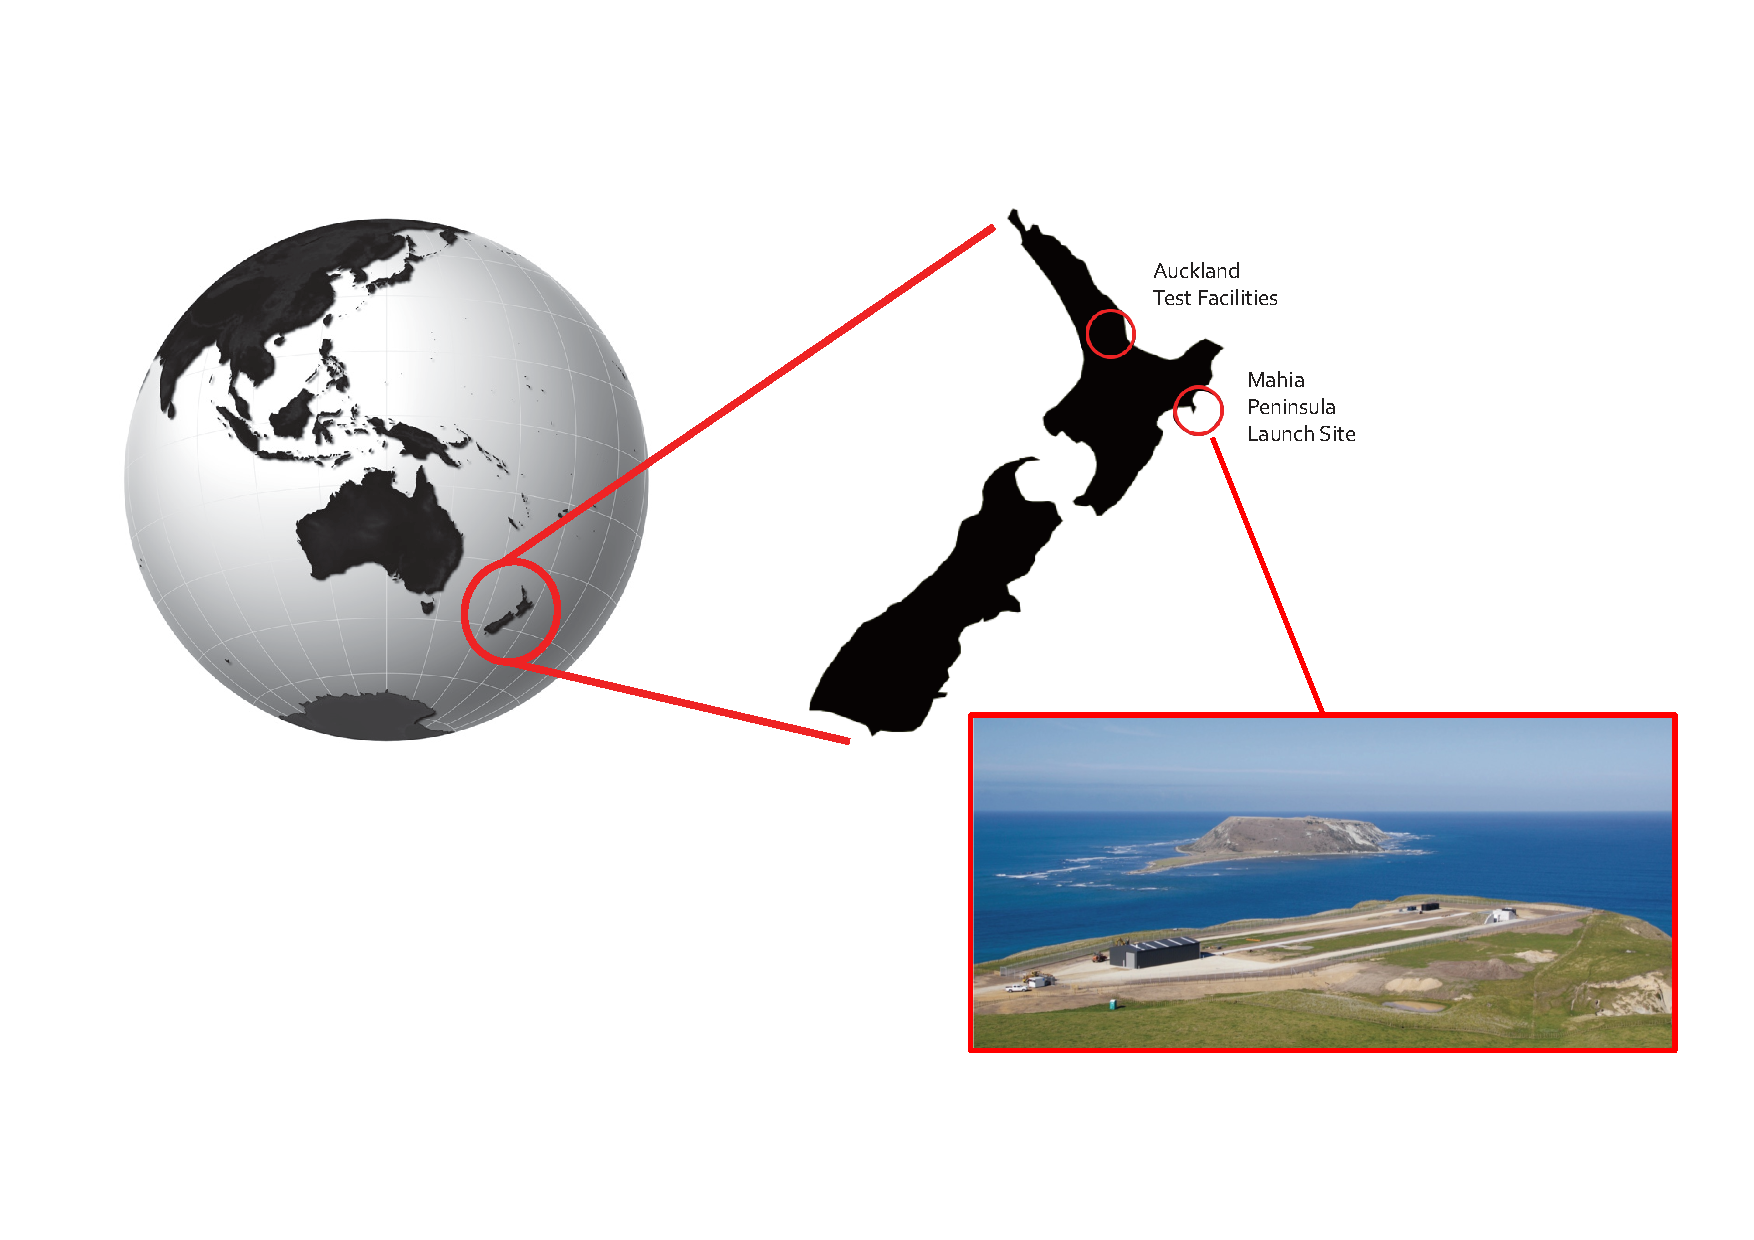
\includegraphics[scale=0.5]{./sections/Constellation_Deployment/S2-Launcher/Images_S2/Picture_4_S2.pdf} 
\caption{Rocket Lab Facilities}
\label{facilities}
\end{figure}
\newline


















%\end{document}